\documentclass[11pt]{article}

\usepackage[margin=1in]{geometry}
\usepackage[T1]{fontenc}
\usepackage{lmodern}
\usepackage{microtype}
\usepackage{amsmath,amssymb,amsthm,mathtools}
\usepackage{mathrsfs}
\usepackage[dvipsnames]{xcolor}
\usepackage[most]{tcolorbox}
\usepackage{tikz}
\usetikzlibrary{decorations.markings,patterns}
\usepackage{enumitem}
\usepackage{tocloft}
\usepackage[hidelinks]{hyperref}

\definecolor{courseblue}{HTML}{1F4E79}
\definecolor{lightblue}{HTML}{EAF2F8}
\definecolor{lightgreen}{HTML}{EAF7EA}
\definecolor{lightpink}{HTML}{FCE8EF}
\definecolor{lightyellow}{HTML}{FFF8D6}
\definecolor{warningyellow}{HTML}{D6A000}
\definecolor{exercisebg}{HTML}{FDEAEA}
\definecolor{exerciseframe}{HTML}{B54040}
\definecolor{examplebg}{HTML}{F4FAFE}
\definecolor{exampleframe}{HTML}{85C1E9}
\definecolor{darkgray}{HTML}{333333}
\definecolor{lightorange}{HTML}{FDEBD8}
\definecolor{orangeframe}{HTML}{E08A3C}
\definecolor{remarkbg}{HTML}{F3EEFB}
\definecolor{remarkframe}{HTML}{9B7FC9}

\setlength{\parindent}{0pt}
\setlength{\parskip}{0.45em}
\setlist[itemize]{topsep=0.25em,itemsep=0.15em}
\renewcommand{\cftsecleader}{\cftdotfill{\cftdotsep}}
\renewcommand{\cftsubsecleader}{\cftdotfill{\cftdotsep}}

\theoremstyle{plain}
\newtheorem{theorem}{Theorem}[section]
\newtheorem{proposition}[theorem]{Proposition}
\newtheorem{lemma}[theorem]{Lemma}
\newtheorem{corollary}[theorem]{Corollary}
\theoremstyle{definition}
\newtheorem{definition}[theorem]{Definition}
\newtheorem{example}[theorem]{Example}
\newtheorem{exercise}[theorem]{Exercise}
\newtheoremstyle{boldremark}
  {3pt}{3pt}{\normalfont}{}{\bfseries}{.}{.5em}
  {\thmname{#1}\thmnumber{ #2}\thmnote{ (#3)}}
\theoremstyle{boldremark}
\newtheorem*{remark}{Remark}
\theoremstyle{remark}
\newtheorem*{fact}{Fact}
\newtheorem*{warning}{Warning}

\tcolorboxenvironment{definition}{
  enhanced,
  unbreakable,
  colback=lightgreen,
  colframe=ForestGreen,
  boxrule=0.7pt,
  arc=2pt,
  left=6pt,
  right=6pt,
  top=5pt,
  bottom=5pt
}

\tcolorboxenvironment{remark}{
  enhanced,
  colback=remarkbg,
  colframe=remarkframe,
  before upper={\setlength{\parskip}{0.5em}},
  boxrule=0.7pt,
  arc=2pt,
  left=6pt,
  right=6pt,
  top=5pt,
  bottom=5pt
}

\tcolorboxenvironment{warning}{
  enhanced,
  colback=lightyellow,
  colframe=warningyellow,
  boxrule=0.7pt,
  arc=2pt,
  left=6pt,
  right=6pt,
  top=5pt,
  bottom=5pt
}

\tcolorboxenvironment{exercise}{
  enhanced,
  colback=exercisebg,
  colframe=exerciseframe,
  boxrule=1pt,
  arc=2pt,
  left=6pt,
  right=6pt,
  top=5pt,
  bottom=5pt
}

\tcolorboxenvironment{example}{
  enhanced,
  colback=examplebg,
  colframe=exampleframe,
  boxrule=0.7pt,
  arc=2pt,
  left=6pt,
  right=6pt,
  top=5pt,
  bottom=5pt
}

\numberwithin{equation}{section}

\newcommand{\be}{\begin{eqnarray}}
\newcommand{\ee}{\end{eqnarray}}
\newcommand{\C}{\mathbb{C}}
\newcommand{\R}{\mathbb{R}}
\newcommand{\N}{\mathbb{N}}
\newcommand{\Z}{\mathbb{Z}}
\DeclareMathOperator{\Log}{Log}
\DeclareMathOperator{\Arg}{Arg}

\DeclareMathOperator{\Hol}{\mathcal{H}\mathrm{ol}}
\DeclareMathOperator{\Real}{Re}
\DeclareMathOperator{\Imag}{Im}
\newcommand{\A}{\mathcal{A}}
\newcommand{\CT}{\C[[T]]}
\newcommand{\CLT}{\C((T))}
\tcbset{breakable}
% Compact spacing around diagrams; keep the main text at 11pt.
\newenvironment{lecturefigure}
 {\par\addvspace{0.25em}\begingroup\setlength{\parskip}{0pt}\centering}
 {\par\endgroup\addvspace{0.25em}}
\begin{document}

\begin{center}
  \colorbox{lightblue}{%
    \begin{minipage}{0.94\textwidth}
      \vspace{0.55em}
      \begin{tabular*}{\textwidth}{@{\extracolsep{\fill}}lr}
        {\color{courseblue}\bfseries\LARGE Lecture 27} &
        {\color{courseblue}\bfseries\LARGE MATH 411}\\[0.35em]
        \textbf{Fall 2026} & \textbf{Date: Nov 20, 2026}\\
        & \textbf{Instructor: Manish Patnaik}
      \end{tabular*}
      \vspace{0.45em}
    \end{minipage}}
\end{center}

\setcounter{tocdepth}{1}
\tableofcontents
\vspace{0.45em}

% Opening section from Lecture 26, Section 5 (handwritten Lecture 25).
\section{Analytic isomorphisms}
\begin{definition}[Analytic isomorphism]
Let $U,V\subseteq\C$ be open. An \emph{analytic isomorphism} from $U$ to $V$
is a bijective holomorphic map $f:U\to V$ whose inverse $g:V\to U$ is also
holomorphic. Equivalently,
\[
 g\circ f=\operatorname{id}_U,\qquad
 f\circ g=\operatorname{id}_V.
\]
We say $U$ and $V$ are \emph{analytically isomorphic} and write $U\cong V$.
The term \emph{biholomorphic} has the same meaning.
\end{definition}

\begin{proposition}\label{prop:analytic-inverse}
Let $U\subseteq\C$ be open and let $f$ be an injective holomorphic function
on $U$. Then $V=f(U)$ is open, and $f:U\to V$ is an analytic isomorphism.
Moreover,
\[
 f'(z)\ne0\quad(z\in U),\qquad
 (f^{-1})'(w)=\frac{1}{f'(f^{-1}(w))}\quad(w\in V).
\]
\end{proposition}

\begin{remark} This result fails over $\R$! Here is a simple example: consider $f(x)=x^3$ on $\R$. It is a bijection with inverse $g(y) = \sqrt[3]{y}$. Now $f'(0)=0$ and this causes the inverse $g(y)$ to be non-differentiable at $0$, since
		$g(y)/y=|y|^{-2/3}\to+\infty$ as $y\to0$.

		What is true is that that for an injective differentiable $f$ on an open subset of $\R$, the
		inverse is differentiable at $f(x_0)$ exactly when $f'(x_0)\ne0$.
		So, for a differentiable inverse on the whole image, we would need to require $f'$ to be
		nowhere zero. This is what follows for free in the holomorphic case.

\end{remark}
We prove this in two steps. First, injectivity forces the derivative to
be nonzero. Then we use a difference quotient to show that the inverse
is holomorphic (this mimics the proof from the real case.)

\subsection{An injective holomorphic map has nonvanishing derivative}

Suppose, for a contradiction, that $f'(z_0)=0$ at some $z_0\in U$.
Injectivity implies that $f$ is nonconstant on the connected component
containing $z_0$. Its analytic expansion therefore has the form
\[
 f(z)=f(z_0)+a(z-z_0)^k+G(z),\qquad a\ne0,\quad k\geq2,
\]
where $G$ vanishes to order at least $k+1$ at $z_0$.
The derivative $f'$ is not identically zero on this component (otherwise
$f$ would be constant there), and hence its zero at $z_0$ is isolated. We can thus
choose $r>0$ small enough that $\overline{D(z_0,r)}\subseteq U$,
\[
 f'(z)\ne0\quad\text{for }0<|z-z_0|\leq r.
\]
Moreover, on the boundary $|z-z_0|=r$ of this same disc, by choosing $r$
perhaps even smaller, we have
\[
 |G(z)| < \frac{|a|}{4}r^k.
\]
Indeed, since $G(z)=(z-z_0)^{k+1}H(z)$ with $H$
holomorphic near $z_0$, choose a bound $M>0$ for $|H|$ on a fixed small
closed disc about $z_0$. Then $|G(z)|\leq Mr^{k+1}$ on the circle of
radius $r$ inside this disc, and the inequality follows for $r<|a|/(4M)$.

We will now use Rouch\'e to contradict injectivity of $f$ as follows: choose a nonzero $\eta\in\C$ with $|\eta|<|a|r^k/4$, and write
\[
 f(z)-f(z_0)-\eta
 =\underbrace{a(z-z_0)^k-\eta}_{F(z)}+G(z).
\]
On $|z-z_0|=r$,
\[
 |F(z)|\geq|a|r^k-|\eta|>\frac{3|a|}{4}r^k>|G(z)|.
\]
The equation $F(z)=0$ is $(z-z_0)^k=\eta/a$. It has exactly $k$ distinct
solutions, all in $D(z_0,r)$, since $0<|\eta/a|<r^k$.
By Rouch\'e's theorem, $f(z)-f(z_0)-\eta$ has exactly $k$ zeros in this
disc, counted with multiplicity.

\begin{lecturefigure}
\begin{minipage}{\linewidth}
\centering
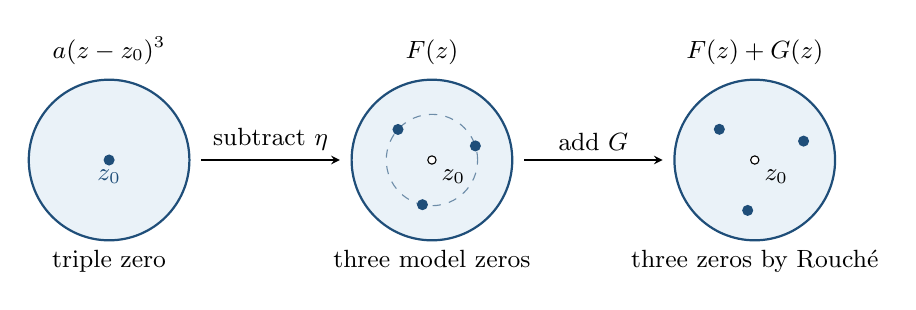
\begin{tikzpicture}[>=stealth,font=\small]
 \foreach \x in {0,4.1,8.2} {
  \filldraw[fill=lightblue,draw=courseblue,thick] (\x,0) circle (1.02);
 }
 \node[above] at (0,1.09) {$a(z-z_0)^3$};
 \node[above] at (4.1,1.09) {$F(z)$};
 \node[above] at (8.2,1.09) {$F(z)+G(z)$};
 \draw[->] (1.17,0) -- node[above] {subtract $\eta$} (2.93,0);
 \draw[->] (5.27,0) -- node[above] {add $G$} (7.03,0);

 \fill[courseblue] (0,0) circle (2pt) node[below] {$z_0$};
 \node[below] at (0,-1.02) {triple zero};
 \begin{scope}[xshift=4.1cm]
  \draw[courseblue!65,dashed] (0,0) circle (0.58);
  \draw[fill=white] (0,0) circle (1.5pt) node[below right] {$z_0$};
  \foreach \angle in {18,138,258} {
   \fill[courseblue] (\angle:0.58) circle (2pt);
  }
  \node[below] at (0,-1.02) {three model zeros};
 \end{scope}
 \begin{scope}[xshift=8.2cm]
  \draw[fill=white] (0,0) circle (1.5pt) node[below right] {$z_0$};
  \foreach \point in {(0.62,0.24),(-0.45,0.39),(-0.09,-0.64)} {
   \fill[courseblue] \point circle (2pt);
  }
  \node[below] at (0,-1.02) {three zeros by Rouch\'e};
 \end{scope}
\end{tikzpicture}
\par\smallskip
{\small Each panel shows $D(z_0,r)$ for $k=3$. Filled dots mark zeros.
The last panel is schematic.}
\end{minipage}
\end{lecturefigure}

None of these zeros equals $z_0$, because $\eta\ne0$. At every such zero
$z$, the derivative is $f'(z)\ne0$ by our choice of $r$. Hence every zero
is simple. There are therefore $k\geq2$ \emph{distinct} points with the
same image $f(z_0)+\eta$, contradicting injectivity. Thus $f'$ never
vanishes on $U$.


\begin{exercise}[The remainder estimate]
With the notation above, write $G(z)=(z-z_0)^{k+1}H(z)$ and bound $H$ on
a fixed small closed disc. Verify that, after shrinking $r$,
$|G(z)|<|a|r^k/4$ on $|z-z_0|=r$.
\end{exercise}

\subsection{The inverse is holomorphic}
On each connected component of $U$, $f$ is nonconstant, since it is
injective. The open mapping theorem on these components shows that
$f$ sends every open subset of $U$ to an open subset of $\C$. In
particular, $V=f(U)$ is open.

Let $g=f^{-1}:V\to U$. Since $f$ is open, $g$ is continuous: for every
open $A\subseteq U$, the inverse image $g^{-1}(A)=f(A)$ is open in $V$.
Fix $w_0\in V$ and set $z_0=g(w_0)$. If $w\ne w_0$ and $z=g(w)$, then
$z\ne z_0$, and
\[
 \frac{g(w)-g(w_0)}{w-w_0}
 =\frac{z-z_0}{f(z)-f(z_0)}
 =\frac{1}{\displaystyle\frac{f(z)-f(z_0)}{z-z_0}}.
\]
As $w\to w_0$, continuity of $g$ gives $z\to z_0$. The denominator tends
to $f'(z_0)\ne0$, so
\[
 g'(w_0)=\frac{1}{f'(z_0)}=\frac{1}{f'(g(w_0))}.
\]
Thus $g$ is complex differentiable at every point of the open set $V$,
hence holomorphic, proving the proposition.


\begin{remark}[Why continuity comes first]
The formal chain rule applied to $g(f(z))=z$ suggests
$g'(f(z))f'(z)=1$. To prove that $g'$ exists, we first use the open mapping
theorem to obtain continuity of $g$, and then take the difference
quotient above.
\end{remark}

\end{document}
